% Aufnahme Data Leakage Prevention in ISO
Im vorherigen Kapitel \ref{threat-kapitel} wurde die Gefahr der versehentlichen Datenoffenlegung in Unternehmen verdeutlicht und die Notwendigkeit effektiver Maßnahmen zur Vermeidung von Datenlecks hervorgehoben. Angesichts der wachsenden Datenmengen und des damit verbundenen Risikos von Datenschutzverletzungen hat sich dieser Bedarf verstärkt. Dies wurde im Jahr 2022 erkannt, als die neueste Version der Norm ISO 27001:2022 die Data Leakage Prevention eingeführt hat. Die internationale Norm ISO 27001 legt die Bedingungen für die Einrichtung, Umsetzung und kontinuierliche Verbesserung eines dokumentierten Informationssicherheitsmanagementsystems fest. Zudem bietet sie Vorschriften für die Beurteilung und Behandlung von Informationssicherheitsrisiken, die an die spezifischen Bedürfnisse jedes Unternehmens angepasst werden müssen \cite{Monev.2023}.

Ein Datenleck kann auf verschiedene Arten auftreten. Obwohl es nicht immer möglich ist, das Auftreten vollständig zu verhindern, können Maßnahmen ergriffen werden, um die Wahrscheinlichkeit zu verringern. Diese Maßnahmen werden als Data Leakage Prevention bezeichnet \cite{Monev.2023}. DLP umfasst eine Vielzahl von Technologien, Produkten und Methoden, die darauf abzielen, zu verhindern, dass vertrauliche Informationen ein Unternehmen unautorisiert verlassen. In den letzten Jahrzehnten wurden verschiedene Sicherheitssysteme wie Firewalls, Intrusion-Detection-Systeme (Einbrucherkennung) und virtuelle private Netzwerke (VPN) eingeführt, um das Risiko von Datenlecks zu reduzieren. Diese Systeme erfüllen ihren Zweck gut, wenn die zu schützenden Daten klar definiert, strukturiert und konstant sind. Jedoch sind sie weniger zuverlässig für Daten, die sich ändern oder unstrukturiert sind.  Eine Firewall kann bspw. den Zugriff auf ein sensibles Datenobjekt durch einfache Regeln verhindern. Allerdings erkennt die Firewall nicht zwangsläufig, wenn dasselbe Datenobjekt über einen E-Mail-Anhang gesendet wird. DLP-Systeme hingegen sind darauf spezialisiert, vertrauliche Daten zu identifizieren, zu überwachen und zu schützen. Sie können so unerwünschte Datenbewegungen effektiver verhindern \cite{Alneyadi.2016}.

Ein DLP-System setzt sich aus einer Vielzahl von Regeln und Richtlinien zusammen, die Daten nach Typ klassifizieren und sicherstellen, dass sie nicht böswillig oder versehentlich verbreitet werden. Das System überwacht die Aktivitäten der Endnutzer, den Datenfluss und die über das Netzwerk übertragenen Informationen. Sobald es verdächtige Aktivitäten entdeckt, löst es eine Systemwarnung aus. DLP-Lösungen identifizieren sensible Inhalte mithilfe von Datenklassifizierungslabels, Inhaltsprüfungsverfahren und Kontextanalysen. Sie überwachen und kontrollieren die Datenaktivitäten nach vordefinierter DLP-Richtlinien. Diese Richtlinien legen fest, ob die Verwendung bestimmter Inhalte oder Daten in bestimmten Situationen zulässig ist \cite{Chugh.2023}.

Gartner klassifiziert DLP-Lösungen in drei Kategorien: Enterprise-DLP-System, integriertes DLP-System, Cloud-natives DLP-System. Eine Enterprise-DLP-Lösung ist ein zentrales System, das darauf ausgelegt ist, komplexe Anforderungen und Strukturen großer Unternehmen zu bewältigen. Sie verfügt über fortschrittliche Technologien zur Identifikation, Klassifizierung und Markierung sensibler Daten und kann verschiedene Datenquellen integrieren. Diese Lösung deckt den gesamten Lebenszyklus von Daten in einem Unternehmen ab, wobei DLP-Richtlinien zentral verwaltet und durchgesetzt werden.
Integrierte DLP-Lösungen hingegen werden direkt in einen Dienst, wie in ein E-Mail-Gateway, integriert und verfügen daher nur über begrenzte Richtlinienfunktionen. Das Management von mehreren integrierten DLP-Systemen erfordert manuellen Aufwand, aber diese Systeme sind speziell an die Anforderungen des jeweiligen Dienstes angepasst und können Inhaltsüberprüfungen effektiver durchführen.
Die dritte Kategorie steht für Cloud-native DLP-Lösungen, die sowohl Software-as-a-Service-Lösungen (SaaS) als auch Cloud-Anbieter mit integrierten DLP-Funktionen umfassen. Sie sind speziell für den Einsatz in Cloud-Umgebungen entwickelt und darauf ausgerichtet, sensible Daten in Cloud-Diensten zu schützen. Diese Lösungen verfügen über Mechanismen zur automatischen Erkennung von sensiblen Daten, die in Cloud-Anwendungen und -Speicherplätzen gespeichert sind, einschließlich der Identifikation von Daten in Form von Dokumenten, E-Mails, Datenbanken und anderen Formaten \cite{Chugh.2023}.
Für die Verhinderung der versehentlichen Offenlegung von sensiblen Daten in der Cloud ist dementsprechend ein Cloud-natives DLP-System die beste Wahl für ein Unternehmen.
Im weiteren Verlauf der Arbeit wird der Begriff DLP-System für alle drei Kategorien verwendet.

% Aufbau / Funktionen
% Bild von NIST oder DLP Funktionen einfügen?
Das Cybersecurity Framework des National Institute of Standards and Technology (NIST CSF) stellt freiwillige Standards und Best Practices bereit, um Unternehmen bei der Verwaltung und Reduzierung von Cybersecurity-Risiken zu unterstützen. Das CSF besteht aus fünf Kernfunktionen, die in Abbildung \ref{f:nist} dargestellt sind: Identifizieren, Schützen, Erkennen, Reagieren und Wiederherstellen.
DLP-Systeme konzentrieren sich hauptsächlich auf die Identifizierung, die Erkennung und den Schutz und ergänzen diese Funktionen durch den Bereich der Überwachung. Die spezifischen Funktionen eines DLP-Systems können je nach Hersteller variieren \cite{NIST.2014}.

\begin{figure}[htbp]
    \centering
    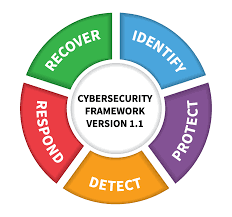
\includegraphics[width=0.6\linewidth]{\figdir/nist.png}
    \caption{NIST Cybersecurity Framework Version 1.1. Quelle: \cite{NIST.2014}.}
    \label{f:nist}
\end{figure}

Die Literaturrecherche hat eine Auswahl an bewährten Methoden ergeben, die in DLP-Systemen vorhanden sein sollten. Um sensible Daten wirksam schützen zu können, ist zunächst die Identifikation erforderlich. Hierbei besteht die Aufgabe darin, ein Dateninventar zu erstellen, die Daten nach ihrer Sensibilität zu klassifizieren und entsprechend zu kennzeichnen. Zum Schutz sensibler Daten sollten Maßnahmen ergriffen werden, die den Zugriff auf die Daten einschränken. Dies beinhaltet die Einführung von Richtlinien wie minimale Zugriffsrechte, starke Authentifizierungsmethoden und strenge Zugriffskontrolllisten. Darüber hinaus sollten Daten sowohl im Ruhezustand als auch während der Übertragung verschlüsselt werden, um sicherzustellen, dass sie für unbefugte Benutzer selbst dann unlesbar bleiben, wenn sie abgefangen werden. Ein DLP-System sollte auch die Datenströme innerhalb und außerhalb des Unternehmens überwachen, um potenzielle Datenschutzverletzungen oder Richtlinienverstöße in Echtzeit zu erkennen. Dies ermöglicht eine schnelle Reaktion auf potenzielle Probleme und begrenzt den daraus resultierenden Schaden \cite{HerreraMontano.2022}\cite{Shishodia.2022}. % es gibt noch weitere Möglichkeiten?

% Herausforderung Daten Klassifizierung
Die Funktionen eines DLP-Systems basieren darauf, dass sensible Daten erkannt und in irgendeiner Art und Weise markiert sind. Der erste Schritt bei DLP-Systemen ist daher die Identifizierung sensibler Daten. Es gibt verschiedene Strategien und Methoden zur Klassifizierung dieser Daten, die durch den Einsatz von KI weiter verbessert wurden.

